% Messwerte: Alle gemessenen Größen tabellarisch darstellen
% Auswertung: Berechnung geforderter Ergebnisse mit Schritten/Fehlerformeln/Erläuterung/Grafik (Programme)
\section{Auswertung}
\label{sec:auswertung}

\begin{table}
	\label{tab:allgemein}
	\centering
	\caption{Allgemeine Messergebnisse.}
		\begin{tabular}
		{S[table-format=1.0]
		 S[table-format=1.0]
		 S[table-format=1.2]}
		\toprule
		{$a \mathbin{/} \unit{\milli\meter}$} & 
		{$b \mathbin{/} \unit{\milli\meter}$} & 
		{$c \mathbin{/} \unit{\milli\meter}$} \\
		\midrule
		1 & 2 & 2.25 \\
		2 & 3 & 3.60 \\
		3 & 4 & 5.00 \\
		4 & 5 & 6.40 \\
 	\bottomrule
	\end{tabular}

\end{table}

\begin{table}
	\label{tab:speziell}
	\centering
	\caption{Spezielle Messergebnisse.}
		\begin{tabular}
		{S[table-format=1.0]
		 S[table-format=1.1]}
		\toprule
		{$a \mathbin{/} \unit{\milli\meter}$} & 
		{$c \mathbin{/} \unit{\milli\meter}$} \\
		\midrule
		1 & 1.4 \\
		2 & 2.8 \\
		3 & 4.2 \\
		4 & 5.7 \\
		5 & 7.1 \\
 	\bottomrule
	\end{tabular}

\end{table}

\begin{figure}[H]
	\label{fig:plot}
	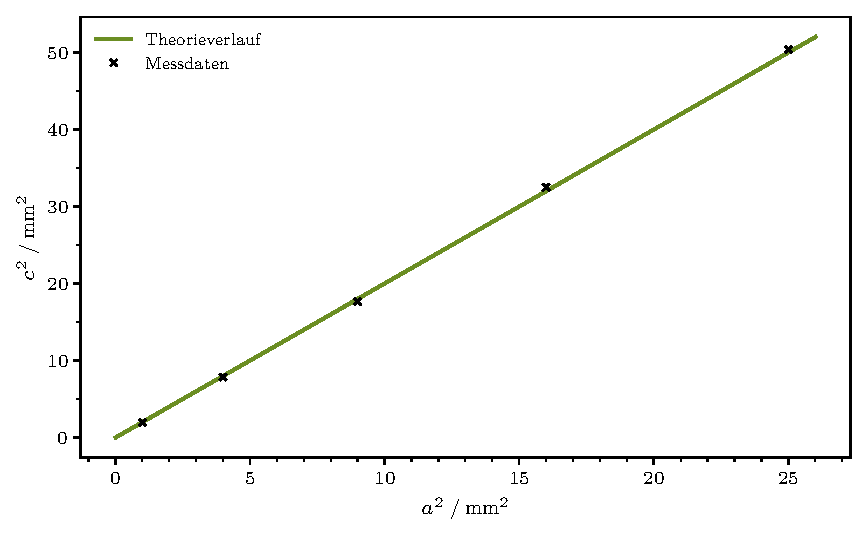
\includegraphics{build/plot.pdf}
	\caption{Messwerte und Theoriegerade.}
\end{figure}

Für $c^2 = ma^2 + n$ liefert \verb+numpy.polyfit+ \cite{numpy}
\begin{align*}
	m = \num{2.03(0.01)} && n = \num{186.1+-2.7}
\end{align*}
als Parameter.
